\documentclass[a4paper, 12pt]{article}
\usepackage[utf8x]{inputenc}
\usepackage[english, russian]{babel}
\usepackage[left=25mm, top=25mm, right=25mm, bottom=25mm]{geometry}
\usepackage{cmap}
\usepackage{indentfirst}
\usepackage{tikz}
\usepackage{float}
\usepackage{amsmath, amsfonts, amssymb}
\usepackage{graphicx}
\usepackage{hyperref}
\usepackage{listings}
\usepackage{caption}
\usepackage{subcaption}
\usepackage{xcolor}
\usepackage{etoolbox}
\usepackage{titlesec}
\usepackage{array}
\pagestyle{plain}
\patchcmd{\tableofcontents}{\contentsname}{\centering\contentsname}{}{}
\titleformat{\section}[block]{\normalfont\large\bfseries\centering}{}{0pt}{}
\titleformat{\subsection}[block]{\normalfont\normalsize\bfseries\centering}{}{0pt}{}
\titleformat{\subsubsection}[block]{\normalfont\small\bfseries\centering}{}{0pt}{}
\allowdisplaybreaks
\graphicspath{{src/images/}}
\usetikzlibrary{patterns}
\definecolor{LightGray}{gray}{0.95}
\definecolor{LightGray2}{gray}{0.7}
\hypersetup{
    colorlinks=true,
    linkcolor=blue,
    filecolor=magenta,
    urlcolor=cyan,
    pdftitle={contents setup},
    pdfpagemode=FullScreen,
}


\begin{document}
    \begin{titlepage}

        \begin{center}
        Федеральное государственное автономное образовательное учреждение высшего образования
        «Национальный Исследовательский Университет ИТМО»
        \vfill
        
        
\includegraphics[width=0.3\textwidth]{itmo.png} % requires /src/images/itmo.png

        {\large\bf ЛАБОРАТОРНАЯ РАБОТА №5}\\
        {\large\bf ПРЕДМЕТ «ЭЛЕКТРОННЫЕ УСТРОЙСТВА СИСТЕМ УПРАВЛЕНИЯ»}\\
        {\large\bf ТЕМА «АКТИВНЫЕ ФИЛЬТРЫ НА ОПЕРАЦИОННЫХ УСИЛИТЕЛЯХ»}\\
        Вариант №10
        \vfill

        \begin{flushright}
            \begin{minipage}{.45\textwidth}
            {
                \hbox{Преподаватель:}
                \hbox{Жданов В. А.}
                \hbox{}
                \hbox{Выполнил:}
                \hbox{Румянцев А. А.}
                \hbox{}
                \hbox{Факультет: СУиР}
                \hbox{Группа: R3341}
                \hbox{Поток: ЭлУСУ R22 бак 1.2}
            }
            \end{minipage}
        \end{flushright}
        \vfill
  
        Санкт-Петербург\\
        2025
        \end{center}
    \end{titlepage}
    
    \tableofcontents

    \newpage
    \section{Цель работы}
    Цель работы -- исследование схем активных фильтров.


    \section{Исходные данные}
    Операционный усилитель берем как в лабораторной работе №3 -- LT1037.


    \subsection{Активные фильтры первого порядка}
    \subsubsection{ФНЧ инвертирующий} \label{sec:lpinv}
    Исходные данные ФНЧ инвертирующий
    \begin{center}
        \begin{tabular}{ | m{3.5em} | m{3.5em}| m{3.5em} | m{2.5em} | m{3.5em} |} 
        \hline
        $R_1$, Ом& $R_2$, Ом &$C_1$, нФ &$K_U^*$ &$f_\text{ср}^*$, кГц\\ 
        \hline
        442.1& 2650 & 10 &6 &6\\ 
        \hline
        \end{tabular}
    \end{center}
    \begin{figure}[H]
        \centering
        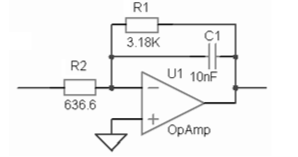
\includegraphics{low_pass_m.png}
        \captionsetup{skip=0pt}
        \caption{Схема ФНЧ инвертирующий}
        \label{fig:null_scheme1}
    \end{figure}
    $$
    K_U=-\dfrac{R_2}{R_1}=-\dfrac{2650}{442.1}\approx-6,
    $$
    $$
    f_\text{ср}=\dfrac{1}{2\pi R_2C_1}=\dfrac{1}{2\pi\cdot2650\cdot10^{-8}}\approx6\text{ кГц};
    $$


    \subsubsection{ФВЧ неинвертирующий} \label{sec:hpninv}
    Исходные данные ФВЧ неинвертирующий
    \begin{center}
        \begin{tabular}{ | m{3.5em} | m{4em}| m{4em} | m{3.5em} | m{2.5em} | m{3.5em} |} 
        \hline
        $R_1$, Ом& $R_2$, кОм &$R_3$, кОм &$C_1$, нФ &$K_U^*$ &$f_\text{ср}^*$, кГц\\ 
        \hline
        3180& 1 &4 &10 &5 &5\\ 
        \hline
        \end{tabular}
    \end{center}
    \begin{figure}[H]
        \centering
        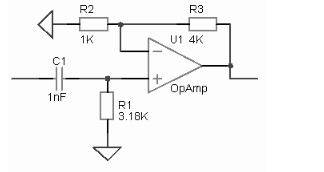
\includegraphics{high_pass_p.png}
        \captionsetup{skip=0pt}
        \caption{Схема ФВЧ неинвертирующий}
        \label{fig:null_scheme2}
    \end{figure}
    $$
    K_U=1+\dfrac{R_3}{R_2}=1+\dfrac{4000}{1000}=5,
    $$
    $$
    f_\text{ср}=\dfrac{1}{2\pi R_1C_1}=\dfrac{1}{2\pi\cdot3180\cdot10^{-8}}\approx5\text{ кГц};
    $$


    \subsection{Активные фильтры второго порядка}
    \subsubsection{ФВЧ Салена-Ки} \label{sec:hpsk}
    Исходные данные ФВЧ Салена-Ки
    \begin{center}
        \begin{tabular}{ | m{3.5em} | m{3.5em}| m{3.5em} | m{4em} | m{4em} | m{4em} | m{2.5em} | m{3.5em} |} 
        \hline
        $C_1$, нФ&$C_2$, нФ&$R_1$, Ом&$R_2$, кОм&$R_3$, кОм&$R_4$, кОм&$K_U^*$&$f_\text{ср}^*$, кГц\\ 
        \hline
        100&100&292.2&0.8766&1&3&4&4\\ 
        \hline
        \end{tabular}
    \end{center}
    \begin{figure}[H]
        \centering
        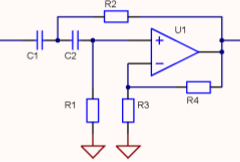
\includegraphics{high_pass_sk.png}
        \captionsetup{skip=0pt}
        \caption{Схема ФВЧ Салена-Ки}
        \label{fig:null_scheme3}
    \end{figure}
    $$
    K_U=1+\dfrac{R_4}{R_3}=1+\dfrac{3}{1}=4,
    $$
    $$
    f_\text{ср}=\dfrac{1}{2\pi\sqrt{\left( R_1R_2C_1C_2 \right)}}=\dfrac{1}{2\pi\sqrt{\left( 292.2\cdot876.6\cdot10^{-14} \right)}}\approx3.145\text{ кГц};
    $$


    \subsubsection{ПФ многопетлевая ОС} \label{sec:strip_multi}
    Исходные данные ПФ многопетлевая ОС
    \begin{center}
        \begin{tabular}{ | m{3.5em} | m{3.5em}| m{3.5em} | m{4em} | m{4em} | m{2.5em} | m{4em} | m{4.5em} |} 
        \hline
        $C_1$, нФ&$C_2$, нФ&$R_1$, Ом&$R_2$, кОм&$R_3$, кОм&$K_U^*$&$f_\text{ср}^*$, кГц &$\Delta f^*$, кГц\\ 
        \hline
        10&10&530.5&4.78&5.3&5&10&6\\ 
        \hline
        \end{tabular}
    \end{center}
    \begin{figure}[H]
        \centering
        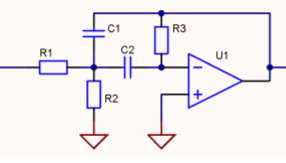
\includegraphics[scale=0.9]{strip_multi.png}
        \captionsetup{skip=0pt}
        \caption{Схема ПФ с многопетлевой обратной связью}
        \label{fig:null_scheme4}
    \end{figure}
    $$
    K_U=\dfrac{R_3}{R_1}\cdot\dfrac{C_2}{C_1+C_2}=\dfrac{5300}{530.5}\cdot\dfrac{10^{-8}}{2\cdot10^{-8}}=\dfrac{R_3}{2R_1}\approx5,
    $$
    $$
    f_\text{ср}=\dfrac{1}{2\pi}\sqrt{\dfrac{1}{R_3C_1C_2}\left( \dfrac{1}{R_1}+\dfrac{1}{R_2} \right)}=\dfrac{1}{2\pi}\sqrt{\dfrac{1}{5300\cdot10^{-16}}\left( \dfrac{1}{530.5}+\dfrac{1}{4780} \right)}\approx10\text{ кГц};
    $$


    \subsubsection{Режекторный фильтр с Т-мостом} \label{sec:rectoring}
    Исходные данные для режекторного фильтра
    \begin{center}
        \begin{tabular}{ | m{3.5em} | m{3.5em}| m{3.5em} | m{4em} | m{4em} | m{3.5em} | m{4em} | m{4em} |} 
        \hline
        $C_1$, нФ&$C_2$, нФ&$C_3$, нФ&$R_1$, кОм&$R_2$, кОм&$R_3$, Ом &$R_4$, кОм&$R_5$, кОм\\ 
        \hline
        10&10&20&0.7958&0.7958&397.9&$\infty$&0\\ 
        \hline
        \end{tabular}
    \end{center}
    \begin{center}
        \begin{tabular}{ | m{3.5em} | m{3.5em}| m{4.5em} |} 
        \hline
        $K_U^*$&$f_\text{ср}^*$, кГц&$\Delta f^*$, кГц\\ 
        \hline
        1&20&20\\ 
        \hline
        \end{tabular}
    \end{center}
    \begin{figure}[H]
        \centering
        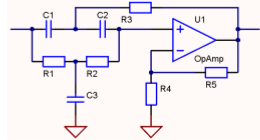
\includegraphics{rectoring.png}
        \captionsetup{skip=0pt}
        \caption{Схема РФ с Т-мостом}
        \label{fig:null_scheme5}
    \end{figure}
    $$
    K_U=1+\dfrac{R_5}{R_4}=1+\dfrac{0}{\infty}=1,
    $$
    $$
    f_\text{ср}=\dfrac{1}{2\pi R_1C_1}=\dfrac{1}{2\pi\cdot795.8\cdot10^{-8}}\approx20\text{ кГц};
    $$


    \section{Исследование активных фильтров первого порядка}
    \subsection{Схема инвертирующего ФНЧ}
    Построим схему инвертирующего ФНЧ в LTspice
    \begin{figure}[H]
        \centering
        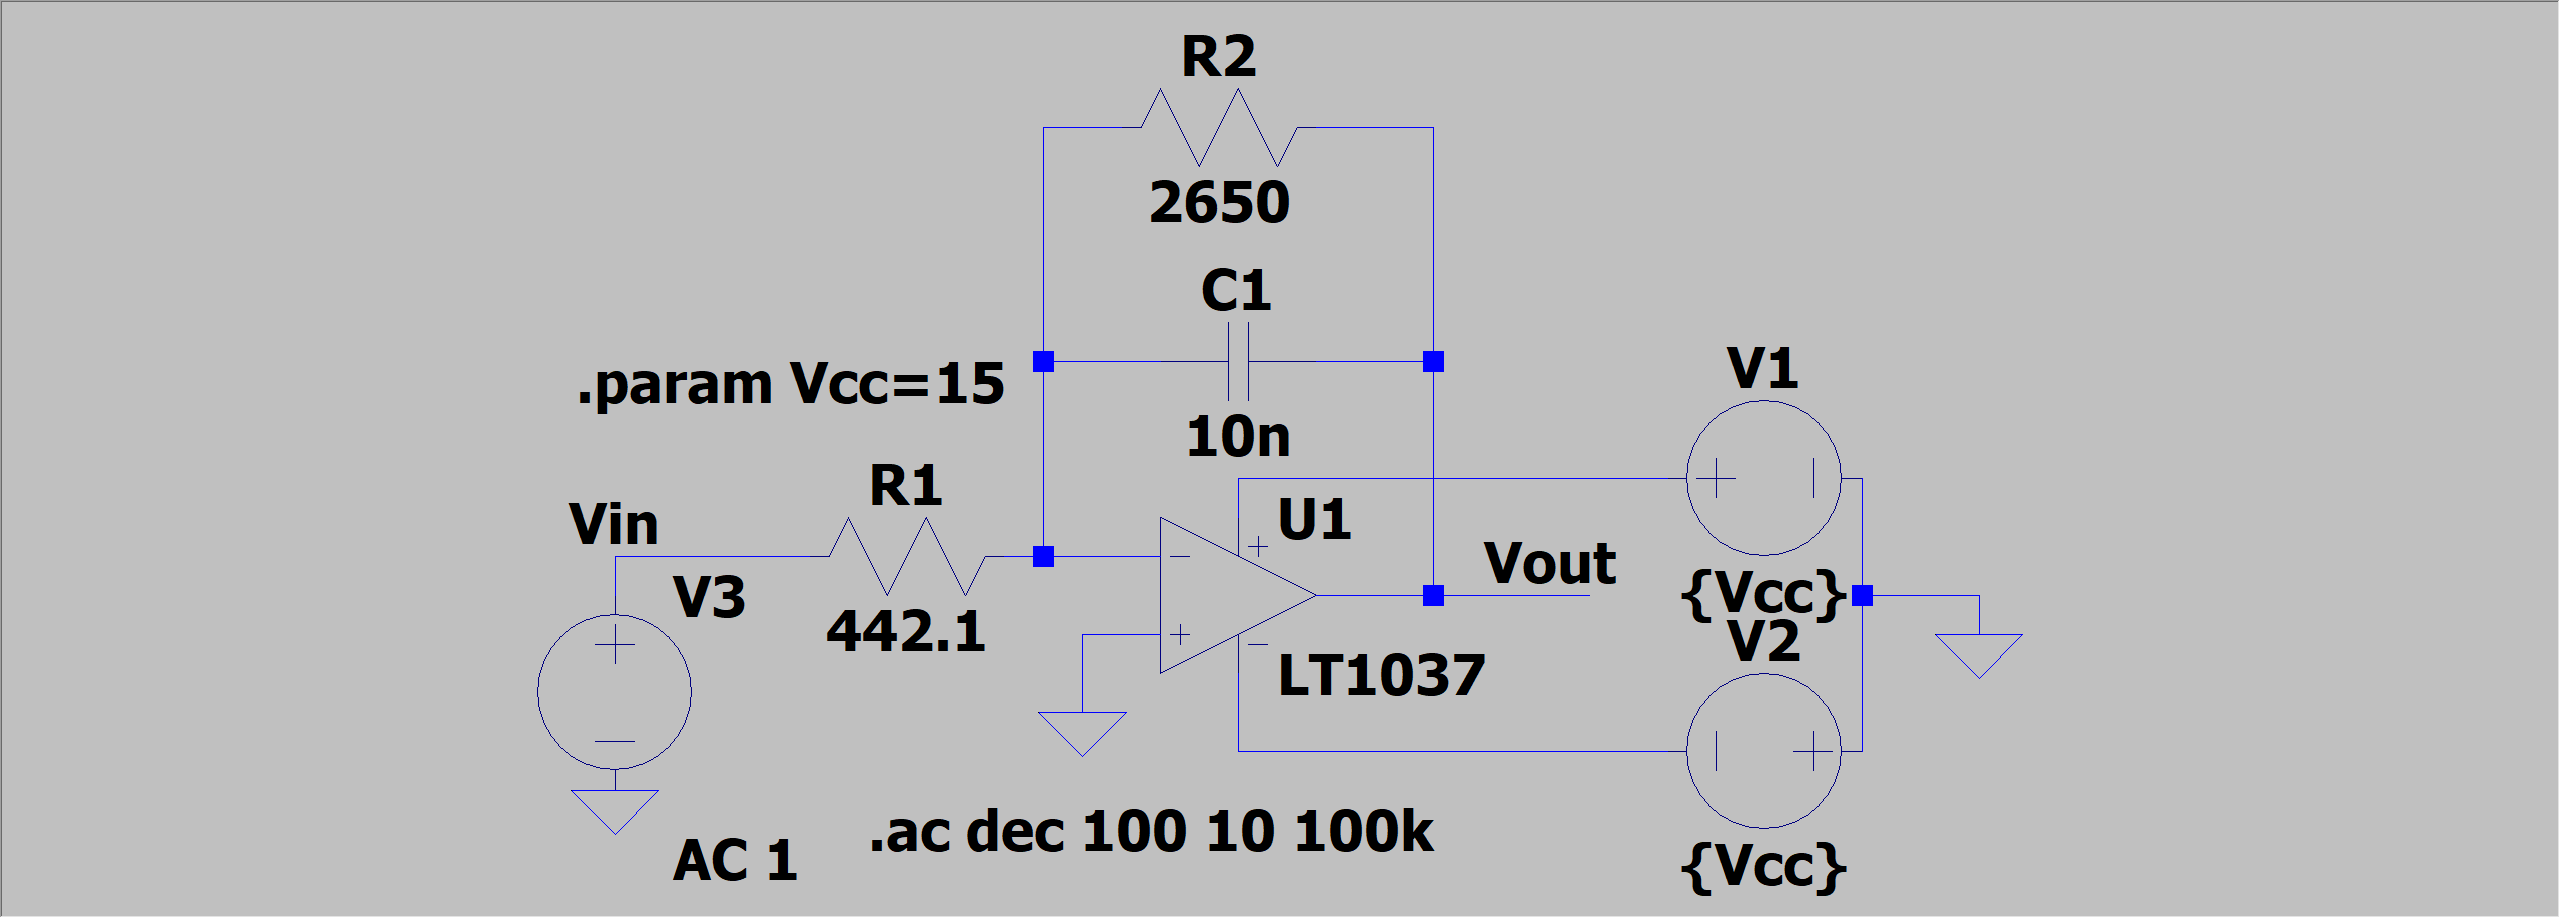
\includegraphics[scale=0.22]{scheme1.png}
        \captionsetup{skip=0pt}
        \caption{Схема инвертирующего ФНЧ}
        \label{fig:scheme1}
    \end{figure}


    \subsection{ЛАФЧХ характеристика инв. ФНЧ}
    Зададим на входной сигнал AC 1 и снимем ЛАЧХ на выходе через .ac dec 100 10 100k (sweep по частоте от 10 Гц до 100 кГц с 100 точками на декаду)
    \begin{figure}[H]
        \centering
        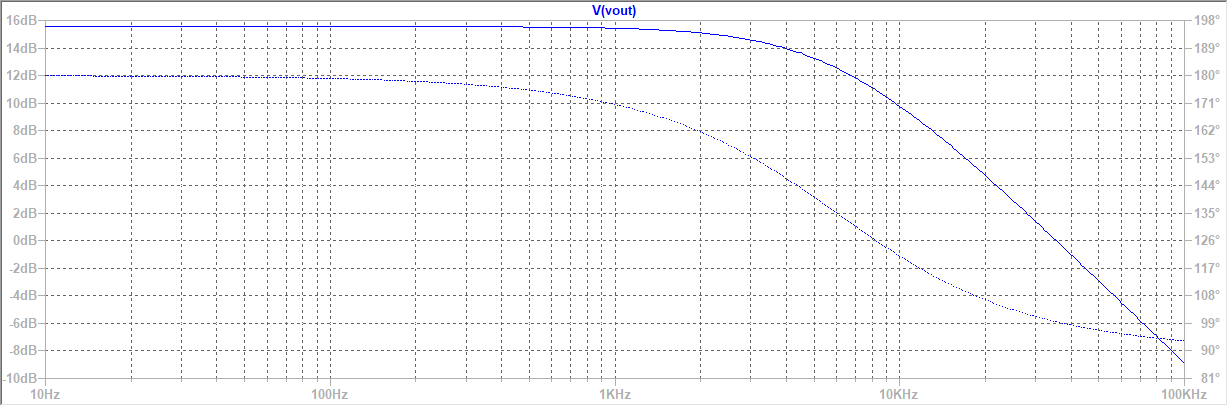
\includegraphics[scale=0.46]{1task_lapfr.png}
        \captionsetup{skip=0pt}
        \caption{ЛАФЧХ характеристика инвертирующего ФНЧ}
        \label{fig:1task_lapfr}
    \end{figure}
    \noindent Курсором снимем значения $A_{n\text{ дБ}},A_{n-3\text{ дБ}},f_{n\text{ дБ}}, f_{n-3\text{ дБ}},\varphi_{n\text{ дБ}}, \varphi_{n-3\text{ дБ}}$,
    где $n-3$ -- амплитуда, на которой находится полоса пропускания фильтра
    \begin{align*}
    &f_{n\text{ дБ}}=10\text{ Гц}:\ A_{n\text{ дБ}}=15.554492\text{ дБ},\ \varphi_{n\text{ дБ}}=179.90453^{\circ};\\
    &f_{n-3\text{ дБ}}=5.9961892 \text{ кГц}:\ A_{n-3\text{ дБ}}=12.548454\text{ дБ},\ \varphi_{n-3\text{ дБ}}=135.02205^{\circ};
    \end{align*}
    Имеем
    $$
    \Delta A=3.006038\text{ дБ},\ f_{n-3\text{ дБ}}=5.9961892\text{ кГц}\approx f_\text{ср}^*=6\text{ кГц};
    $$
    То есть полоса пропускания
    $$
    0\leq f\leq 5.9961892\text{ кГц}
    $$
    Экспериментально полученная полоса пропускания фильтра совпадает с теоретиески расчитанной (см. $f_\text{ср}^*$ в табл. \ref{sec:lpinv}).


    \subsection{Схема неинвертирующего ФВЧ}
    Построим схему неинвертирующего ФВЧ в LTspice
    \begin{figure}[H]
        \centering
        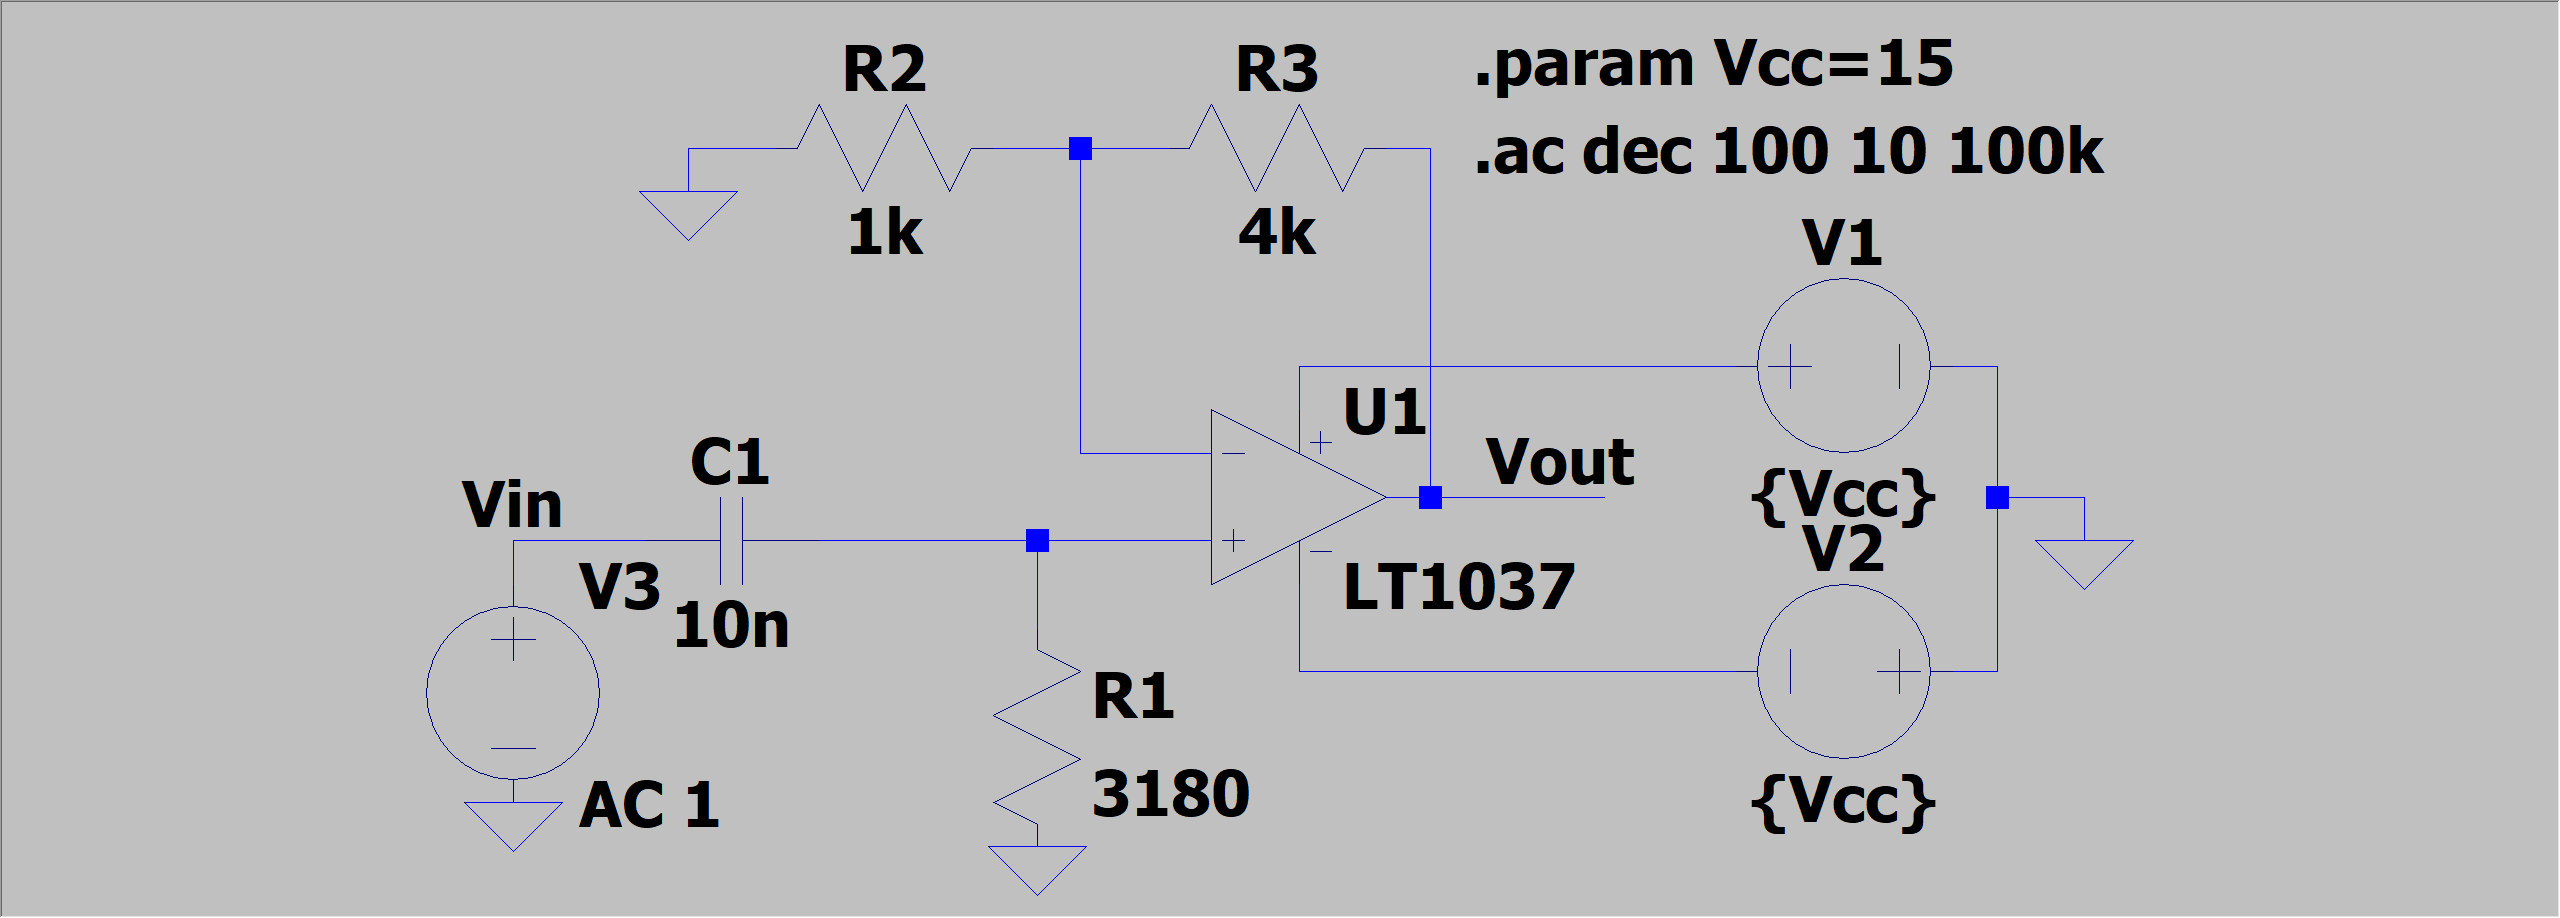
\includegraphics[scale=0.22]{scheme2.png}
        \captionsetup{skip=0pt}
        \caption{Схема неинвертирующего ФВЧ}
        \label{fig:scheme2}
    \end{figure}


    \subsection{ЛАФЧХ характеристика неинв. ФВЧ}
    Аналогично найдем ЛАФЧХ характеристику фильтра
    \begin{figure}[H]
        \centering
        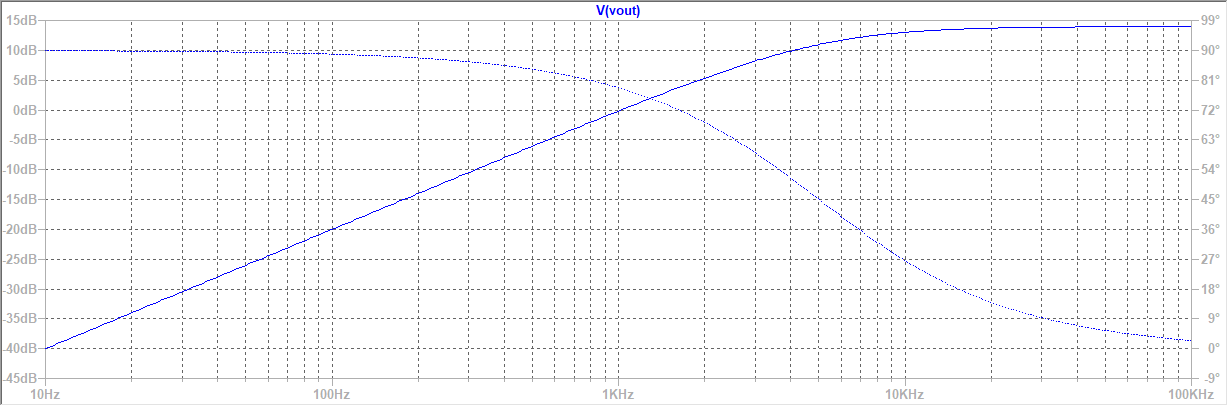
\includegraphics[scale=0.46]{2task_lapfr.png}
        \captionsetup{skip=0pt}
        \caption{ЛАФЧХ характеристика неинвертирующего ФВЧ}
        \label{fig:2task_lapfr}
    \end{figure}
    \noindent Аналогично курсором снимем значения
    \begin{align*}
    &f_{n\text{ дБ}}=100\text{ кГц}:\ A_{n\text{ дБ}}=13.977885\text{ дБ},\ \varphi_{n\text{ дБ}}=2.4062551^{\circ};\\
    &f_{n-3\text{ дБ}}=5.0300312 \text{ кГц}:\ A_{n-3\text{ дБ}}=10.990257\text{ дБ},\ \varphi_{n-3\text{ дБ}}=44.830656^{\circ};
    \end{align*}
    Имеем
    $$
    \Delta A=2.987628\text{ дБ},\ f_{n-3\text{ дБ}}=5.0300312\text{ кГц}\approx f_\text{ср}^*=5\text{ кГц};
    $$
    То есть полоса пропускания
    $$
    5.0300312\leq f\leq100\text{ кГц}
    $$
    Экспериментально полученная полоса пропускания фильтра совпадает с теоретиески расчитанной (см. $f_\text{ср}^*$ в табл. \ref{sec:hpninv}).


    \section{Исследование активных фильтров второго порядка}
    \subsection{ФВЧ Салена-Ки}
    Построим схему одноименного фильтра в LTspice
    \begin{figure}[H]
        \centering
        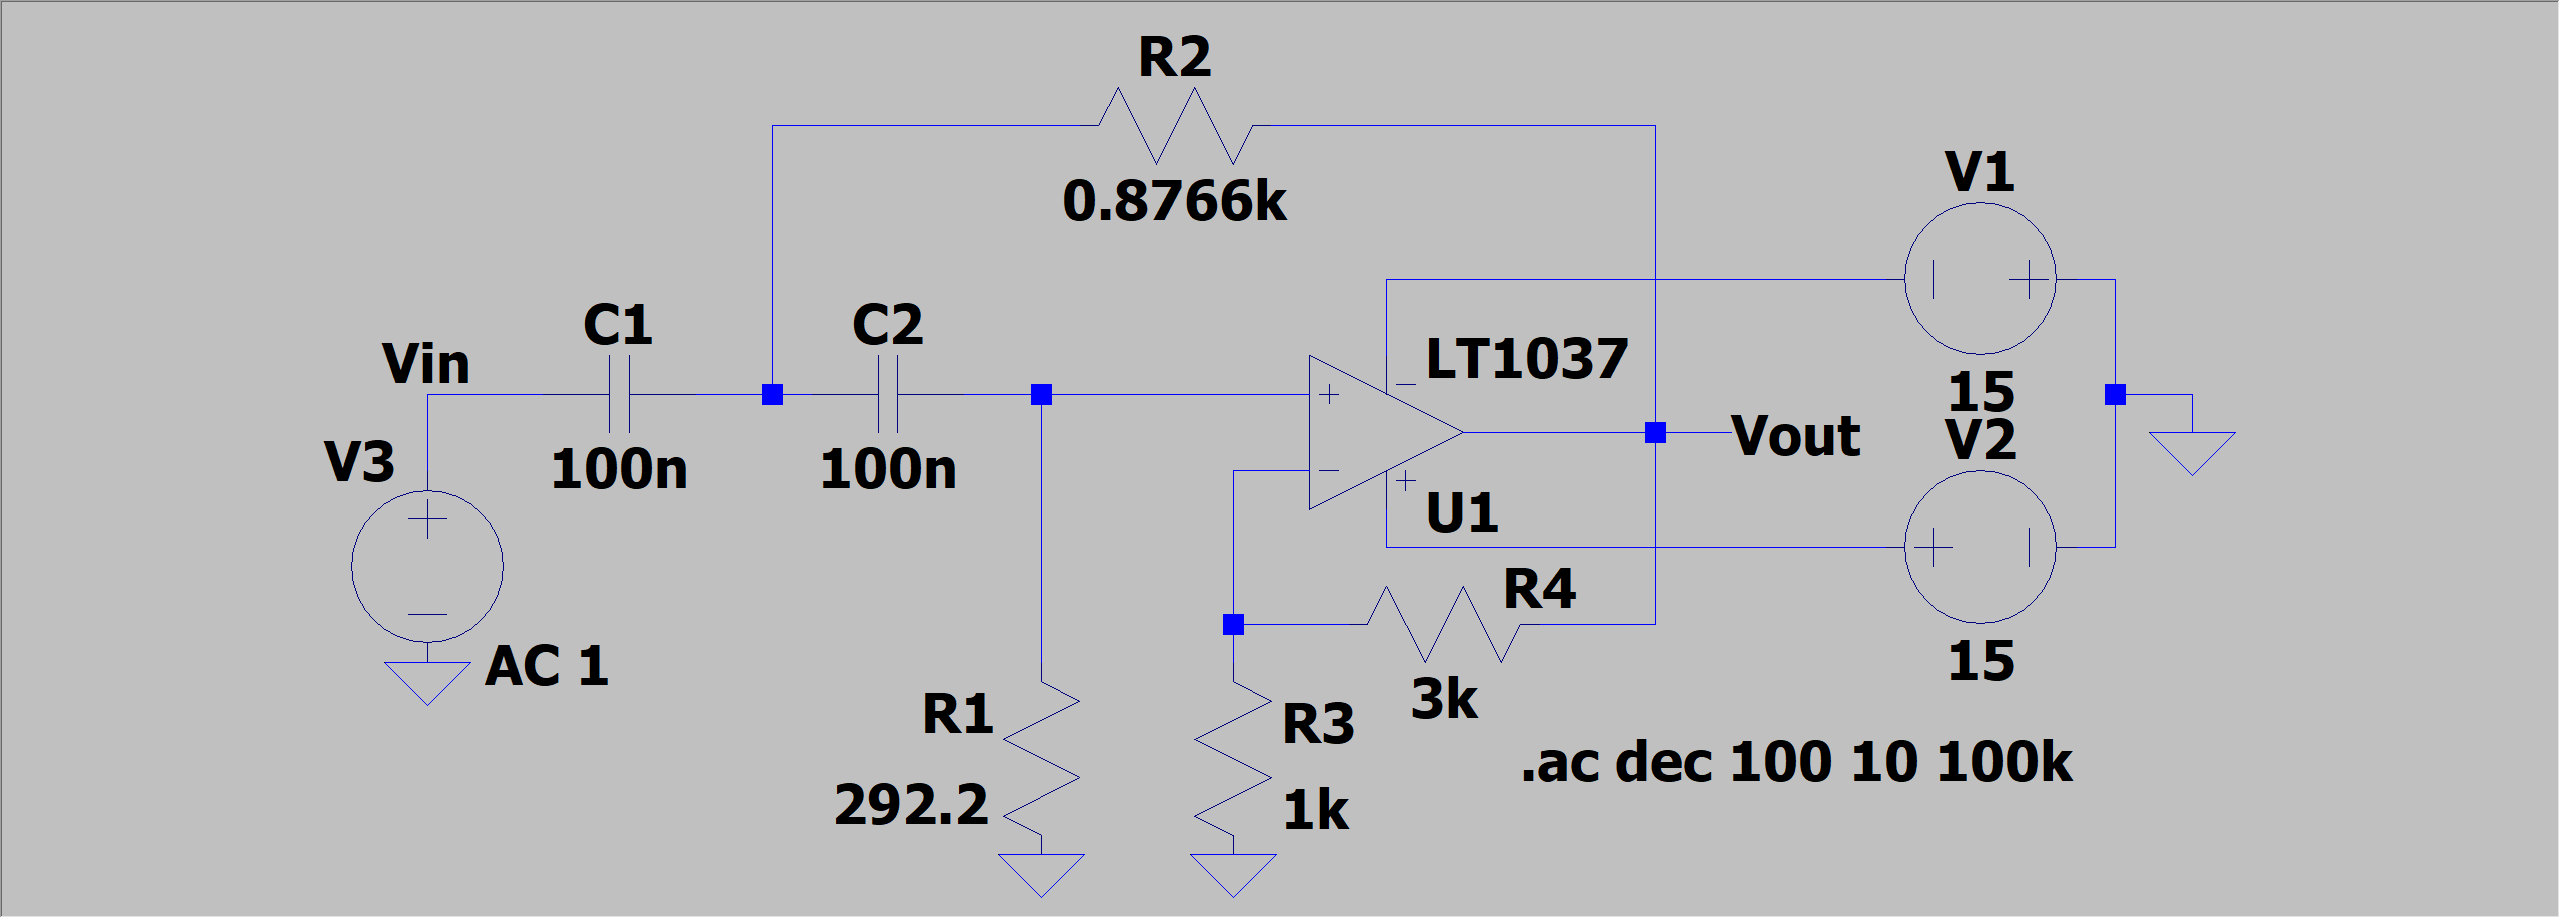
\includegraphics[scale=0.22]{scheme3.png}
        \captionsetup{skip=0pt}
        \caption{Схема ФВЧ Салена-Ки}
        \label{fig:scheme3}
    \end{figure}


    \subsection{ЛАФЧХ характеристика ФВЧ Салена-Ки}
    Аналогично найдем ЛАФЧХ характеристику фильтра
    \begin{figure}[H]
        \centering
        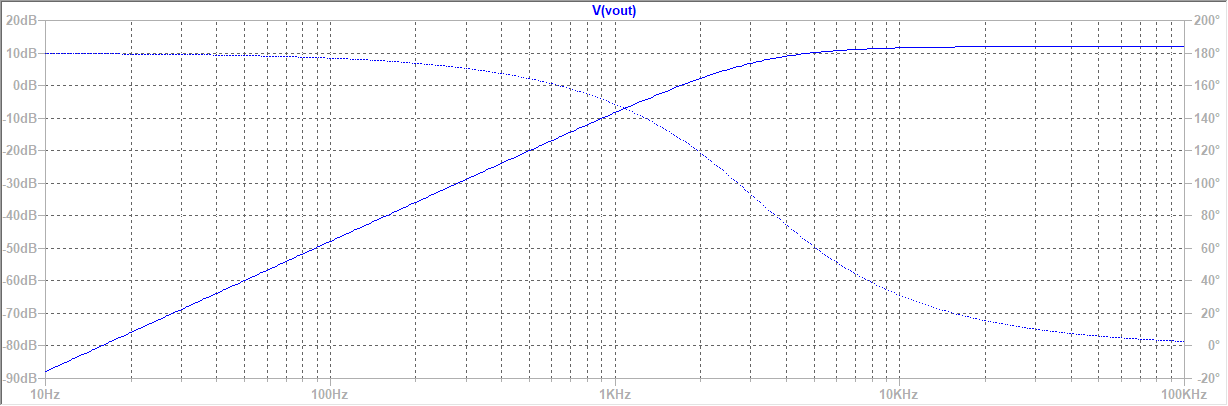
\includegraphics[scale=0.46]{3task_lapfr.png}
        \captionsetup{skip=0pt}
        \caption{ЛАФЧХ характеристика ФВЧ Салена-Ки}
        \label{fig:3task_lapfr}
    \end{figure}
    \noindent Аналогично курсором снимем значения
    \begin{align*}
    &f_{n\text{ дБ}}=100\text{ кГц}:\ A_{n\text{ дБ}}=12.041278\text{ дБ},\ \varphi_{n\text{ дБ}}=2.728094^{\circ};\\
    &f_{n-3\text{ дБ}}=4.0088442 \text{ кГц}:\ A_{n-3\text{ дБ}}=9.0426662\text{ дБ},\ \varphi_{n-3\text{ дБ}}=74.15903^{\circ};
    \end{align*}
    Имеем
    $$
    \Delta A=2.9986118\text{ дБ},\ f_{n-3\text{ дБ}}=4.0088442\text{ кГц}\approx f_\text{ср}^*=4\text{ кГц};
    $$
    То есть полоса пропускания
    $$
    4.0088442\leq f\leq100\text{ кГц}
    $$
    Экспериментально полученная полоса пропускания фильтра совпадает с теоретиески расчитанной (см. $f_\text{ср}^*$ в табл. \ref{sec:hpsk}).


    \subsection{ПФ многопетлевая ОС}
    Построим схему одноименного фильтра в LTspice
    \begin{figure}[H]
        \centering
        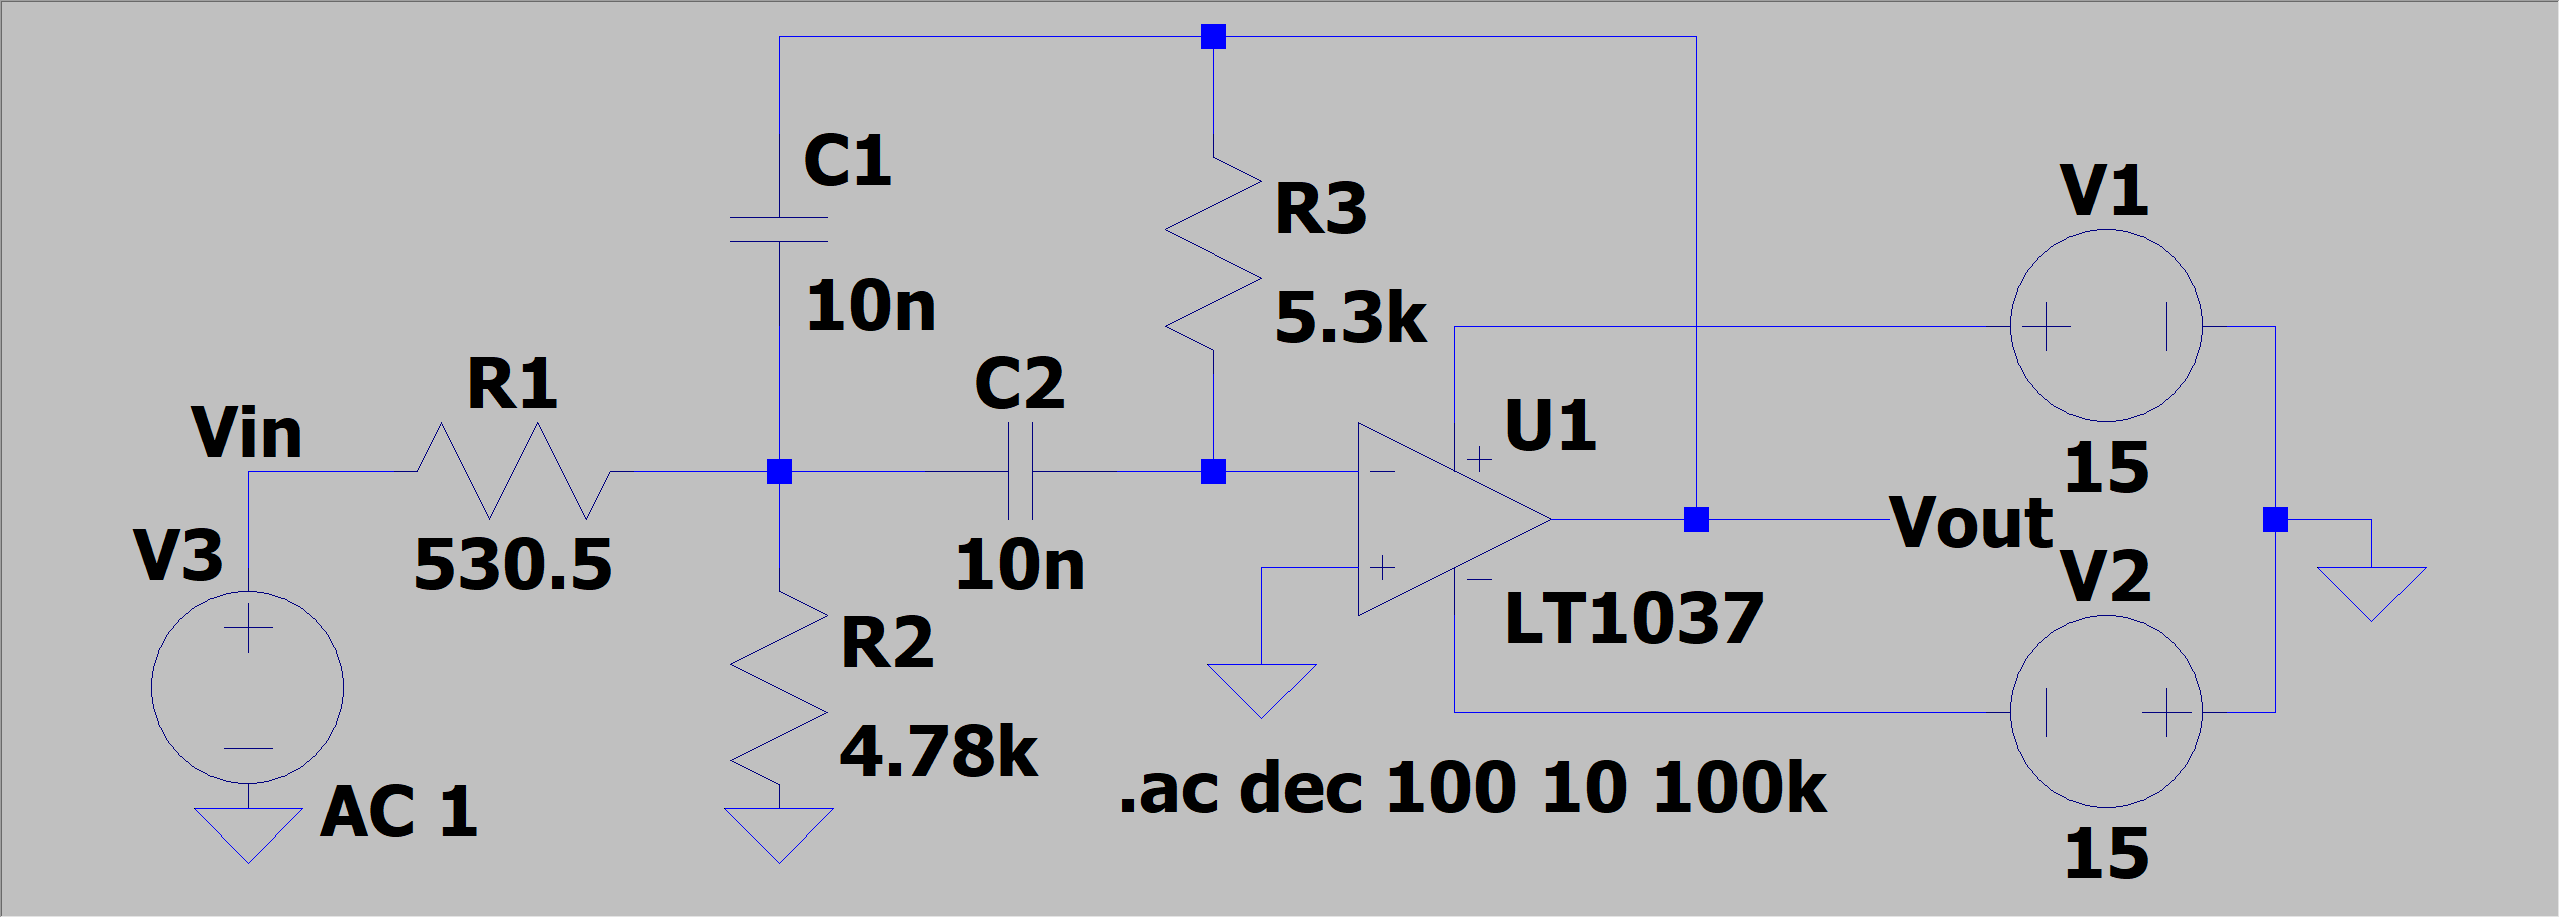
\includegraphics[scale=0.22]{scheme4.png}
        \captionsetup{skip=0pt}
        \caption{Схема ПФ с многопетлевой обратной связью}
        \label{fig:scheme4}
    \end{figure}


    \subsection{ЛАФЧХ характеристика ПФ многопетлевая ОС}
    Аналогично найдем ЛАФЧХ характеристику фильтра
    \begin{figure}[H]
        \centering
        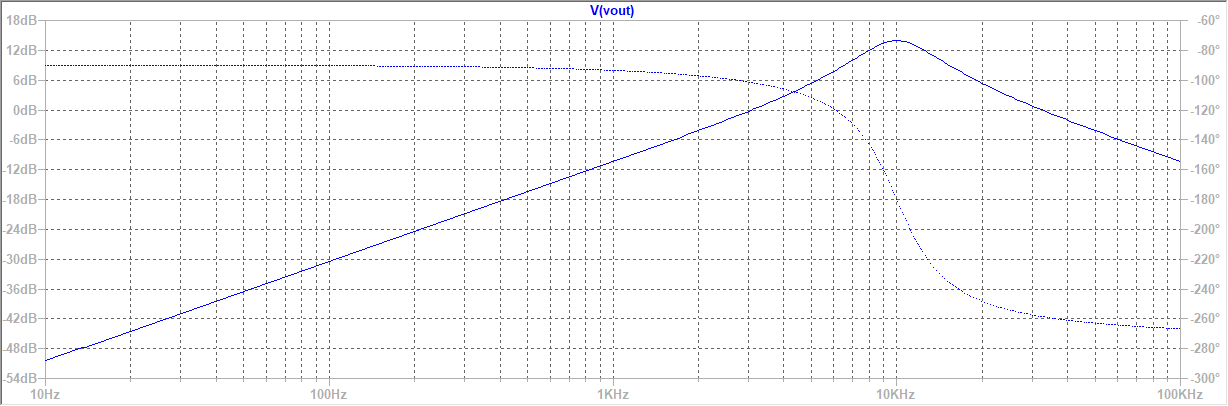
\includegraphics[scale=0.46]{4task_lapfr.png}
        \captionsetup{skip=0pt}
        \caption{ЛАФЧХ характеристика ПФ многопетлевая ОС}
        \label{fig:4task_lapfr}
    \end{figure}
    \noindent Курсором измерим вершину <<горы>> и значения слева и справа от нее
    \begin{align*}
    &f_{n\text{ дБ}}=9.9797335\text{ кГц}:\ A_{n\text{ дБ}}=13.969476\text{ дБ},\ \varphi_{n\text{ дБ}}=-179.59242^{\circ};\\
    &f_{n-3\text{ дБ сл}}=7.4515513 \text{ кГц}:\ A_{n-3\text{ дБ сл}}=10.982289\text{ дБ},\ \varphi_{n-3\text{ дБ сл}}=-135.16323^{\circ};\\
    &f_{n-3\text{ дБ спр}}=13.474586 \text{ кГц}:\ A_{n-3\text{ дБ спр}}=10.926412\text{ дБ},\ \varphi_{n-3\text{ дБ спр}}=-225.242^{\circ};
    \end{align*}
    Имеем
    $$
    \Delta A_\text{сл}=A_{n\text{ дБ}}-A_{n-3\text{ дБ сл}}=2.987187\text{ дБ},
    $$
    $$
    \Delta A_\text{спр}=A_{n\text{ дБ}}-A_{n-3\text{ дБ спр}}=3.043064\text{ дБ};
    $$
    $$
    f_{n\text{ дБ}}=9.9797335\text{ кГц}\approx f_\text{ср}^*=10\text{ кГц},
    $$
    $$
    \Delta f_{n-3\text{ дБ}}=f_{n-3\text{ дБ спр}}-f_{n-3\text{ дБ сл}}=6.0230347\text{ кГц}\approx \Delta f^*=6\text{ кГц};
    $$
    То есть полоса пропускания
    $$
    7.4515513\leq f\leq13.474586\text{ кГц},\ f_\text{ср}=9.9797335\text{ кГц}, \Delta f=6.0230347\text{ кГц};
    $$
    Экспериментально полученная полоса пропускания фильтра совпадает с теоретиески расчитанной (см. $f_\text{ср}^*,\Delta f^*$ в табл. \ref{sec:strip_multi}).


    \subsection{Режекторный фильтр}
    Построим схему одноименного фильтра в LTspice
    \begin{figure}[H]
        \centering
        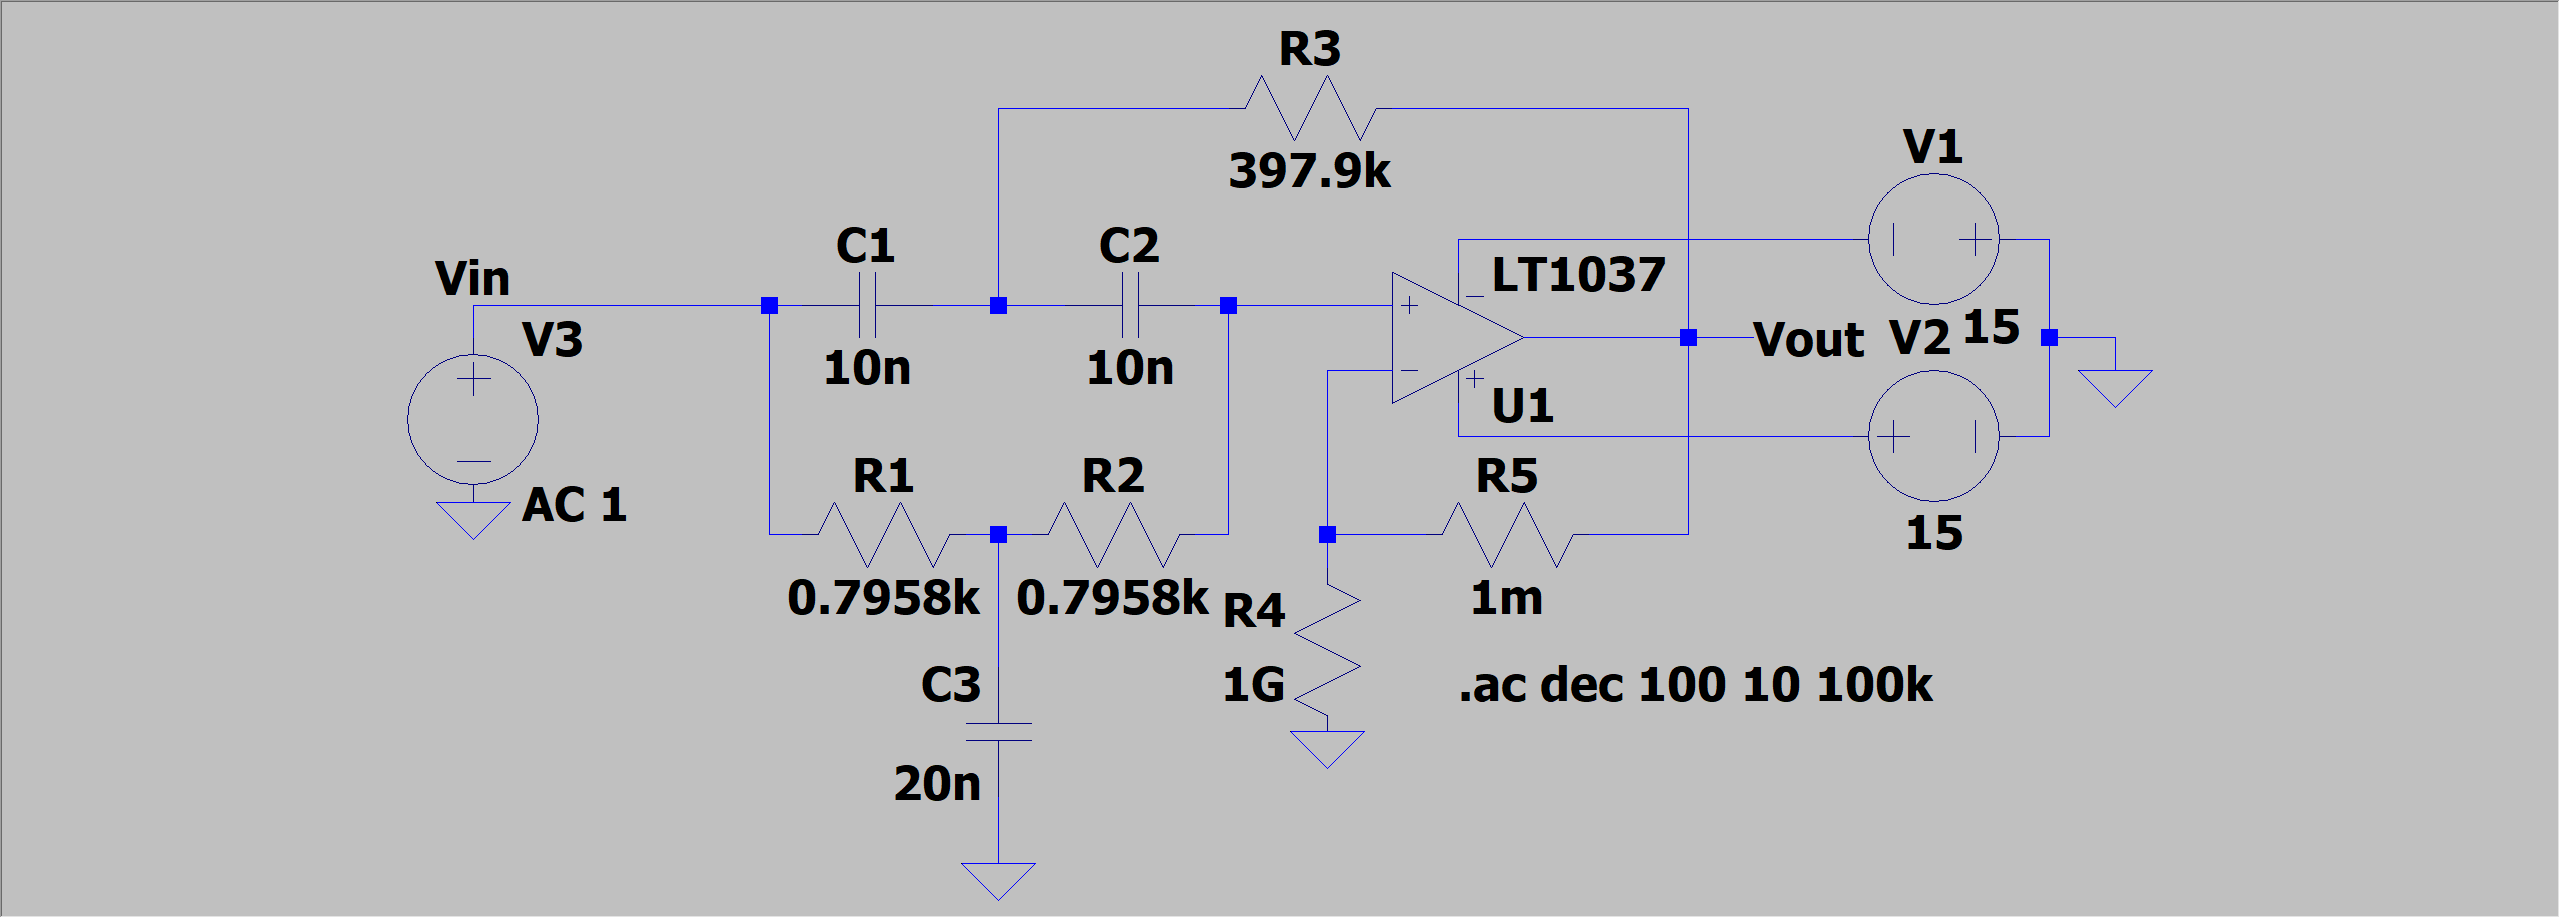
\includegraphics[scale=0.22]{scheme5.png}
        \captionsetup{skip=0pt}
        \caption{Схема РФ с Т-мостом}
        \label{fig:scheme5}
    \end{figure}


    \subsection{ЛАФЧХ характеристика РФ с Т-мостом}
    Аналогично найдем ЛАФЧХ характеристику фильтра
    \begin{figure}[H]
        \centering
        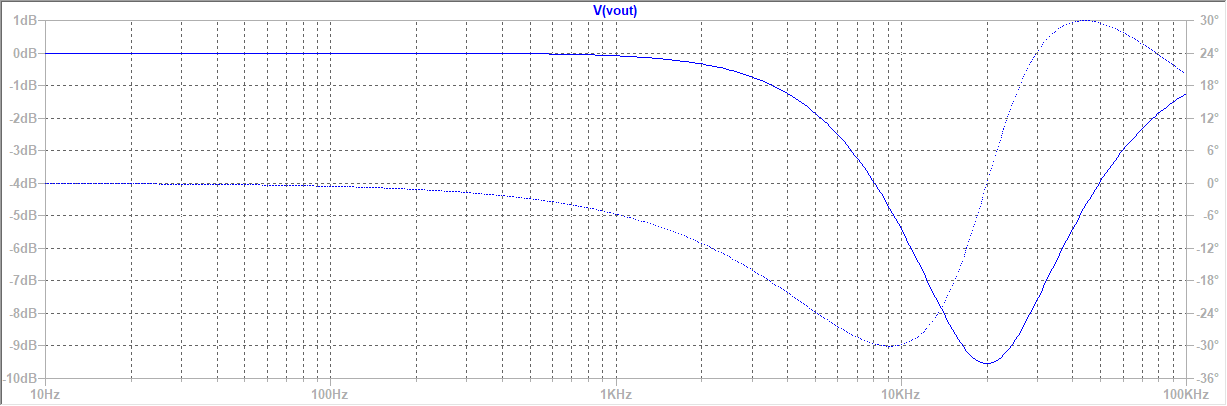
\includegraphics[scale=0.46]{5task_lapfr.png}
        \captionsetup{skip=0pt}
        \caption{ЛАФЧХ характеристика РФ с Т-мостом}
        \label{fig:5task_lapfr}
    \end{figure}
    \noindent Фаза была отрицательной, стала положительной -- наблюдаем смену полярности.
    Курсором измерим низину <<ямы>> и значения слева и справа от нее
    \begin{align*}
        &f_{n\text{ дБ}}=20.061636\text{ кГц}:\ A_{n\text{ дБ}}=-9.5470452\text{ дБ},\ \varphi_{n\text{ дБ}}=0.25264918^{\circ};\\
        &f_{n-3\text{ дБ сл}}=11.587212 \text{ кГц}:\ A_{n-3\text{ дБ сл}}=-6.4971049\text{ дБ},\ \varphi_{n-3\text{ дБ сл}}=-28.006004^{\circ};\\
        &f_{n-3\text{ дБ спр}}=34.454665 \text{ кГц}:\ A_{n-3\text{ дБ спр}}=-6.5038859\text{ дБ},\ \varphi_{n-3\text{ дБ спр}}=27.939365^{\circ};
    \end{align*}
    Имеем
    $$
    \Delta A_\text{сл}=|A_{n\text{ дБ}}-A_{n-3\text{ дБ сл}}|=3.0499403\text{ дБ},
    $$
    $$
    \Delta A_\text{спр}=|A_{n\text{ дБ}}-A_{n-3\text{ дБ спр}}|=3.0431593\text{ дБ};
    $$
    $$
    f_{n\text{ дБ}}=20.061636\text{ кГц}\approx f_\text{ср}^*=20\text{ кГц},
    $$
    $$
    \Delta f_{n-3\text{ дБ}}=f_{n-3\text{ дБ спр}}-f_{n-3\text{ дБ сл}}=22.867453\text{ кГц}\approx \Delta f^*=20\text{ кГц};
    $$
    То есть полоса пропускания
    $$
    \begin{cases}
        0\leq f<11.587212 \text{ кГц},\\
        34.454665<f\leq100\text{ кГц},
    \end{cases} f_\text{ср}=20.061636\text{ кГц},\ \Delta f=22.867453\text{ кГц};
    $$
    Экспериментально полученная полоса пропускания фильтра совпадает с теоретиески расчитанной (см. $f_\text{ср}^*,\Delta f^*$ в табл. \ref{sec:rectoring}).


    \section{Вывод}
    В ходе выполнения работы были рассмотрены различные виды
    активных фильтров первого и второго порядков. Были построены
    схемы и промоделированы ЛАФЧХ для каждого случая. Результаты
    подтверждают корректность расчетов.
\end{document}